\documentclass[handout]{beamer}

\usepackage[utf8]{inputenc} % Language and font encoding
\usepackage[icelandic]{babel}
\usepackage[T1]{fontenc}


\usepackage{tikz}
\usepackage[listings,theorems]{tcolorbox}
\usepackage{booktabs}
\usepackage{minted} %Minted and configuration
\usemintedstyle{default}

\renewcommand{\theFancyVerbLine}{\sffamily \arabic{FancyVerbLine}}
%%%%%%%%%%%
% More math
%%%%%%%%%%%
\newcommand{\Mod}[1]{\ \text{mod}\ #1}

%%%%%%%%%%%%%%%%%%%%%%
% Beamer configuration
%%%%%%%%%%%%%%%%%%%%%%
\setbeamertemplate{navigation symbols}{}
\usecolortheme{dove}
\setbeamercolor{frametitle}{fg=white}

\usebackgroundtemplate%
{%
\vbox to \paperheight{

\includegraphics[width=\paperwidth]{Pics/hi-slide-head-2016}

\vfill
\hspace{0.5cm}
\includegraphics[width=0.3\paperwidth]{Pics/hi-von-logo}
\vspace{0.4cm}
    }%
}

\AtBeginSection[]
{
  \begin{frame}<beamer>
    \frametitle{Yfirlit}
    \tableofcontents[currentsection]
  \end{frame}
}

\setbeamerfont{frametitle}{size=\normalsize}
\addtobeamertemplate{frametitle}{}{\vspace*{0.5cm}}

%%%%%%%%%%%%%%%%%%%%%%%%%
% tcolorbox configuration
%%%%%%%%%%%%%%%%%%%%%%%%%

% Setup from: http://tex.stackexchange.com/a/43329/21638
\tcbset{%
    noparskip,
    colback=gray!10, %background color of the box
    colframe=gray!40, %color of frame and title background
    coltext=black, %color of body text
    coltitle=black, %color of title text 
    fonttitle=\bfseries,
    alerted/.style={coltitle=red, colframe=gray!40},
    example/.style={coltitle=black, colframe=green!20, colback=green!5},
}


%%%%%%%%%%%%%%%%%%%%%%%
% Further configuration
%%%%%%%%%%%%%%%%%%%%%%%
\hypersetup{colorlinks=true,pdfauthor={Eirikur Ernir Thorsteinsson},linkcolor=blue,urlcolor=blue}
\graphicspath{{./Pics/}}

\author{Eiríkur Ernir Þorsteinsson}
\institute{Háskóli Íslands}
\date{Haust 2016}

\title{Tölvunarfræði 1a}
\subtitle{Vika 3, fyrri fyrirlestur}

\begin{document}

\begin{frame}
\titlepage
\end{frame}

\section{Inngangur}

\begin{frame}{Í síðasta þætti\ldots}
\begin{itemize}
 \item Vigrar og fylki
 \item Aðgerðir á vigra og fylki
 \begin{itemize}
  \item Stakvísar aðgerðir vs. aðgerðir úr línulegri algebru
  \item Depilfeldi og krossfeldi
 \end{itemize}
 \item Rökvigrar
 \begin{itemize}
  \item Rökvísanir
 \end{itemize}
\end{itemize}
\end{frame}

\begin{frame}{Matlab-leyfi}
\begin{itemize}
 \item Nokkur ykkar hafa lent í vandræðum með Matlab-leyfi
 \item Séuð þið beðin um \emph{activation key}:
 \begin{itemize}
  \item \texttt{05226-45858-01826-26094-59607}
 \end{itemize}
 \item Séuð þið beðin um \emph{file installation key}:
 \begin{itemize}
  \item R2016a: {\scriptsize \texttt{21138-57626-18349-64703-45527-05546-36337-15390-27602-18969-28816 } }
  \item R2015b : {\scriptsize \texttt{48568-38634-00620-27726-05580-48643-44090-25848-24305-28470-14612 } }
 \end{itemize}
\end{itemize}
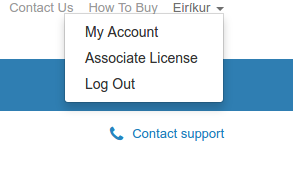
\includegraphics[width=0.3\textwidth]{license}
\end{frame}


\begin{frame}{Forrit í Matlab}
\begin{itemize}
 \item Hingað til höfum við verið að fást við einstakar skipanir
 \item En til að gera \emph{forrit} þurfum við meira
 \item Gerðir Matlab-forrita:
 \begin{itemize}
  \item Skipanaskrár (e. \emph{scripts})
  \begin{itemize}
   \item Runa Matlab-skipana geymdar í \texttt{.m} skrám
  \end{itemize}
  \item Notendaskilgreind föll (e. \emph{user-defined functions})
  \begin{itemize}
   \item Föll sem reikna út og skila gildi (líkt og innbyggð föll gera)
  \end{itemize}
 \end{itemize}
\end{itemize}
\end{frame}

\section{Reiknirit (3.1)}

\begin{frame}{Reiknirit}
\begin{itemize}
 \item Reiknirit (e. \emph{algorithm}) er lýsing á aðferð til að leysa verkefni
 \begin{itemize}
  \item Þarf að vera nógu nákvæm til að hægt sé að skrifa forrit eftir henni
  \item Oft skrifuð á mannamáli
  \item Lýsinguna má svo útfæra (e. \emph{implement}) í forritunarmáli
 \end{itemize}
\end{itemize}
\end{frame}

\begin{frame}[fragile]{Reiknirit: Að finna minnsta stak}
\begin{columns}
\column{0.7\textwidth}
Setja fyrsta stakið sem það minnsta\\
Síðan \textbf{fyrir öll} hin stökin i í vigrinum\\
\quad \textbf{Ef} stak i er minna en það minnsta hingað til\\
\qquad Setja stak i sem minnsta stakið
\column{0.3\textwidth}
\begin{minted}[frame=lines]{matlab}
>> v = [4, 3, 5];
>> min(v)
ans =  3
\end{minted}
\end{columns}
\vspace{1cm}
Alvöru reiknirit, á íslensku. Engu að síður er ákveðið skipulag á lýsingunni.
\end{frame}

\begin{frame}{Eitt verkefni - mörg reiknirit}
\begin{itemize}
 \item Röðun n-staka vigurs er vel þekkt vandamál
 \begin{itemize}
  \item Til yfir hundrað ólík reiknirit fyrir röðun
  \item Það er ekkert eitt besta reikniritið
  \item Þau hafa sín sérkenni og henta fyrir mismunandi gerðir gagna
 \end{itemize}
\end{itemize}
\end{frame}

\begin{frame}{Nokkur röðunarreiknirit}
\begin{itemize}
 \item Innsetningarröðun
 \begin{itemize}
  \item Svipað og við notum oft við að raða spilum á hendi
  \item Tökum eitt spil í einu og setjum það á réttan stað í raðaða hlutanum
 \end{itemize}
 \item Valröðun
 \begin{itemize}
  \item Finna stærsta gildið og setja það aftast
  \item Finna síðan næststærsta og setja það næstaftast, o.s.frv.
 \end{itemize}
 \item Quicksort
 \begin{itemize}
  \item Skipta listanum í tvennt eftir vendistaki (pivot)
  \item Láta öll stök minni en pivot-inn framar, öll stærri en pivot-inn aftar
  \item Raða síðan hvorum hluta fyrir sig Quicksort\footnote{Þessi lausnaraðferð kallast \emph{endurkvæm}}
 \end{itemize}
\end{itemize}
\end{frame}

\begin{frame}{Hermun röðunarreiknirita}
\begin{itemize}
 \item Vefsíða með hermun á nokkrum reikniritum
 \begin{itemize}
  \item \url{http://www.sorting-algorithms.com/}
 \end{itemize}
 \item Hljóð og röðun:
 \begin{itemize}
  \item \url{https://www.youtube.com/watch?v=kPRA0W1kECg}
 \end{itemize}
 \item Með dansi!
 \begin{itemize}
  \item \url{http://www.youtube.com/watch?v=ROalU379l3U}
 \end{itemize}
\end{itemize}
\end{frame}

\begin{frame}{Fyrirlestraræfing}
Skráið ykkur inn á \url{http://socrative.com/} og gerið fyrstu spurninguna

Herbergisnúmer = \texttt{TOL105G2016}

Notendanafn = HÍ-tölvupóstfang

Reiknirit:

\vspace{0.5cm}
 Gefinn er vigur $v$ af tölum og tala $x$\\
 Skoðum hverja tölu í $v$.\\
 \textbf{Ef} talan í sæti $i$ er jöfn $x$\\
 \quad skila i
\end{frame}

\section{Undir Húddinu (3.2)}

\subsection{Æðri forritunarmál og vélarmál}
\begin{frame}{Tölvuforrit}
 \begin{itemize}
  \item Nefnt hefur verið að tölvur vinni með ``bita'' af upplýsingum
  \item Örgjörvar tölva ``skilja'' aðeins vélarmál (e. \emph{machine language})
  \begin{itemize}
   \item Mjög frumstæðar skipanir:
   \begin{itemize}
    \item Leggja gildið í hólfi 48 við gildið í hólfi 32
    \item Ef gildið í hólfi 104 er núll halda keyrslu áfram í hólfi 1008
   \end{itemize}
   \item Erfitt að forrita í vélarmáli (tímafrekt og hætta á villum)
  \end{itemize}
    \item Vélamál, bitar og önnur frumstæð vinnsla eru þó venjulega víðs fjarri í nútímaforritun, t.d. með Matlab
  \begin{itemize}
   \item Matlab er ``æðra forritunarmál'' (e. \emph{high level programming language})
  \end{itemize}
 \end{itemize}
\end{frame}

\begin{frame}{Frá æðra máli til vélarmáls}
\begin{itemize}
 \item Æðri forritunarmál eru nær mennskum hugsunarhætti
 \item Til að breyta forritskóða í æðra forritunarmáli í vélamálskóða eru tvær lausnir:
 \begin{enumerate}
  \item Þýðing (e. \emph{compilation})
  \begin{itemize}
   \item Forriti í æðra máli breytt í jafngilt forrit í vélarmáli sem heild
  \end{itemize}
  \item Túlkun (e. \emph{interpretation})
  \begin{itemize}
   \item Forrit í æðra máli keyrt línu fyrir línu af túlki
  \end{itemize}
 \end{enumerate}
\end{itemize}
\end{frame}

\subsection{Þýðing og túlkun}
\begin{frame}{Þýðing}
\begin{columns}
\column{0.5\textwidth}
\begin{itemize}
 \item Forritið keyrt í gegnum þýðanda (e. \emph{compiler})
 \item Fáum út keyrslukóða (e. \emph{executable}), þ.e. einhvers konar .exe-skrá
 \item Þýðandinn getur skoðað allt forritið til að búa til hraðvirkan keyrslukóða (optimization)
\end{itemize}
\column{0.5\textwidth}
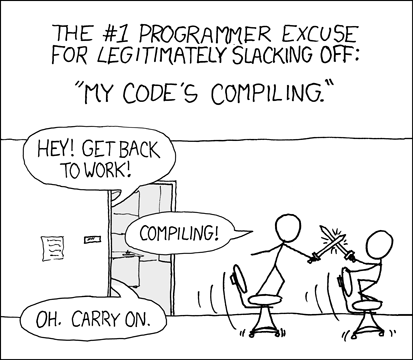
\includegraphics[width=\linewidth]{Pics/compiling}\\
Þýðing á stórri forritsskrá getur tekið dágóðan tíma (\href{https://xkcd.com/303/}{xkcd})
\end{columns}
\end{frame}

\begin{frame}{Túlkun}
\begin{itemize}
 \item Túlkur er forrit sem framkvæmir annað forrit línu fyrir línu
 \begin{itemize} 
  \item Túlkurinn sér aðeins eina línu (eða fáar línur) í einu
  \item Keyrsla er hægari en á þýddu forriti, hver lína er í raun þýdd á keyrslutíma
 \end{itemize}
 \item Auðvelt er að bjóða upp á keyrslu skipun-fyrir-skipun í túlkuðu máli
\end{itemize}
\end{frame}

\begin{frame}{Þýtt vs. túlkað}
\begin{itemize}
 \item Sum mál eru alltaf\footnote{Svo kennarinn viti til\ldots} túlkuð
 \begin{itemize}
  \item Javascript, PHP, Perl, \ldots
 \end{itemize}
  \item Sum forritunarmál eru alltaf þýdd
 \begin{itemize}
  \item C++, C, Fortran, \ldots
 \end{itemize}
 \item Engu að síður er forritunarmál ekki þýtt eða túlkað í eðli sínu
 \begin{itemize}
  \item Oft er ekki ómögulegt að skrifa þýðanda fyrir forritunarmál sem venjulega er túlkað, og öfugt
  \item Hugmyndir um ``forritunarmál'' og ``skriptumál'' sem aðskilda hluti eru oft byggðar á misskilningi
 \end{itemize}
 \item Sum mál eru ýmist þýdd eða túlkuð
 \item Sum eru bæði þýdd og túlkuð!
\end{itemize}
\end{frame}

\begin{frame}{Þýðing OG túlkun}
\begin{itemize}
 \item Sum forritunarmál eru þýdd yfir á millimál (intermediate language) og millimálið er túlkað
 \begin{itemize}
  \item Kostir:
  \begin{itemize}
   \item Þýðandinn sér allt forritið og getur bestað millikóðann
   \item Millimálið er einskonar vélarmál fyrir sýndarvél (e. \emph{virtual machine})
  \end{itemize}
  \item Gallar:
  \begin{itemize}
   \item Millimálið er ennþá túlkað og keyrsla er því hægvirkari en á þýddu forrit
  \end{itemize}
 \end{itemize}
 \item Þetta er mjög algeng aðferð
\end{itemize}
\end{frame}

\begin{frame}{Dæmi um þýðingu og túlkun}
\begin{itemize}
 \item Forritunarmálið Java
 \begin{itemize}
  \item Þýðandinn (javac) þýðir yfir á Java bætakóða
  \item Keyrsluumhverfi (Java virtual machine) framkvæmir bætakóðann
 \end{itemize}
\end{itemize}
\begin{itemize}
 \item Forritunarmálið C\#
 \begin{itemize}
  \item Þýðandinn (MS Visual C\#) þýðir yfir á CIL (Common Intermediate Language)
  \item Keyrsluumhverfi (.NET CLR) framkvæmir CIL forritið
 \end{itemize}
\end{itemize}
\end{frame}

\begin{frame}{JIT þýðandi}
\begin{itemize}
 \item Matlab hefur JIT (Just-In-Time) þýðanda
 \item Skipanir eru þýddar yfir í vélarmál á keyrslutíma
 \begin{itemize}
  \item Ef sama skipunin er keyrð oft (í lykkju\footnote{Við förum yfir lykkjur seinna}) þá keyrist hún á vélarmálshraða eftir fyrsta skiptið
  \item Ekki notað fyrir allar skipanir (helst einfaldar lykkjur)
  \item Gerist algerlega sjálfkrafa (``á bakvið tjöldin'')
 \end{itemize}
 \item Keyrsluhraði Matlab-kóða er oft sambærilegur við keyrsluhraða þýdds kóða
\end{itemize}
\end{frame}

\begin{frame}{Fyrirlestraræfing}
Skráið ykkur inn á \url{http://socrative.com/} og gerið næstu spurningu

Herbergisnúmer = \texttt{TOL105G2016}

Notendanafn = HÍ-tölvupóstfang
\end{frame}

\section{Skipanaskrár (3.2)}

\begin{frame}{Skipanaskrár í matlab}
\vspace{\baselineskip}
\begin{columns}
\column{0.8\textwidth}
\begin{itemize}
 \item Passa að núverandi skráarsvæði (Current Folder) sé rétt stillt (mikilvægt!)
 \item Til að búa til nýja skipanaskrá má ýta á takka í Matlab-viðmótinu (sjá til hliðar), eða ýta á CTRL + N, eða slá inn \texttt{edit skráarnafn} í skipanaglugga
 \item Nafnviðauki Matlab-skipanaskráa er \texttt{.m}
 \item Það að búa til skipanaskrá opnar ritil
 \begin{itemize}
  \item Þar má slá inn Matlab-skipanir (muna að vista)
 \end{itemize}
 \item Til að keyra skipanaskrá má slá inn nafn hennar í skipanaglugga
\end{itemize}
\column{0.2\textwidth}

\includegraphics{Pics/new-script}
\end{columns}
\end{frame}

\begin{frame}{Skipanaskrár - dæmi}
\begin{columns}
\column{0.5\textwidth}
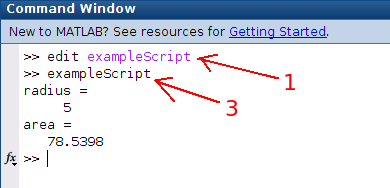
\includegraphics[width=\linewidth]{Pics/script-create-3}
\column{0.5\textwidth}
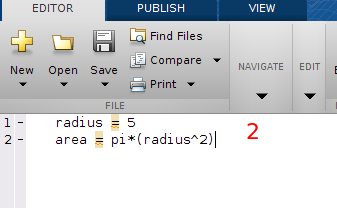
\includegraphics[width=\linewidth]{Pics/script-create-2}
\end{columns}
\end{frame}

\subsection{Athugasemdir (3.2.1)}

\begin{frame}[fragile]{Athugasemdir}
\begin{itemize}
 \item Getum sett inn athugasemdir (comments) í skipanaskrár
 \item Texti sem lýsir því sem skipanirnar gera
 \item Athugasemdir eru ekki keyrðar
 \item Athugasemd í Matlab byrjar á \%
 \item Athugasemd getur verið fremst í línu eða fyrir aftan skipun
\end{itemize}
\begin{minted}[frame=lines]{matlab}
% Þetta er athugasemd
summa = 0     % Upphafsstilla summu
\end{minted}
\end{frame}

\begin{frame}[fragile]{Skjölun skipanaskráa}
\vspace{\baselineskip}
Venja er í Matlab að fyrsta línan í skipanaskrá lýsi henni.
\begin{minted}[frame=lines]{matlab}
% Þessi skrá reiknar flatarmál hrings

radius = 5;
area = pi * (radius^2);
\end{minted}
Þá má fá upplýsingar með skipuninni \texttt{help}
\begin{minted}[frame=lines]{matlab}
>> help exampleScript
  Þessi skrá reiknar flatarmál hrings
\end{minted}
\end{frame}

\section{Notendaskilgreind föll (3.7)}

\begin{frame}{Notendaskilgreind föll}
\begin{itemize}
 \item Höfum séð mörg innbyggð föll í Matlab
 \begin{itemize}
  \item \texttt{sin, cos, abs, max,} \ldots
 \end{itemize}
 \item Sjáum nú hvernig á að skilgreina ný föll
 \item Þau hegða sér eins og innbyggðu föllin
 \item Ath: Í stærðfræði tengir fall saman gildi þannig að fyrir hvert inntaksgildi er nákvæmlega eitt úttaksgildi (Ef $f(a) = b$ þá gildir ekki að $f(a) = c$). Misjafnt er hversu vel þetta á við um föll í daglegri forritun.
\end{itemize}
\end{frame}

\begin{frame}{Föll í forritun}
\begin{itemize}
 \item Í forritun:
 \begin{itemize}
  \item Föll oftast notuð til að framkvæma tiltekna útreikninga sem byggja á inntaksgildum
  \item Útkoma útreikninganna er eitt gildi
 \end{itemize}
 \item Dæmi:
 \begin{itemize}
  \item Fall til að finna flatarmál kúlu
  \item Fall sem breytir frá Fahrenheit í Celsíus
  \item Fall til að finna stærsta samdeili tveggja heiltalna
 \end{itemize}
\end{itemize}
\end{frame}

\begin{frame}[fragile]{Skilgreining falla í Matlab}
Almennt snið falla:
\begin{minted}[frame=lines]{matlab}
function skilabreyta = nafn(stiki1, stiki2, ...)
   skipanir
end
\end{minted}
Dæmi (sett í skrá \texttt{calculateArea.m}):
\begin{minted}[frame=lines]{matlab}
function area = calculateArea(radius)
% calculateArea reiknar flatarmál hrings út frá radíus
% Notkun:  calculateArea(radius)

   area = pi * radius*radius;
end
\end{minted}

\end{frame}

\begin{frame}[fragile]{Notkun falla}
Notendaskilgreind föll eru notuð á sama hátt og innbyggð föll
\begin{minted}[frame=lines]{matlab}
>> calculateArea(4)
ans =
   50.2655
\end{minted}
Algengt mynstur er að nota skipanaskrár til að kalla á föll. Þá eru útreikningar framkvæmdir í falli, en gögn sótt eða skilgreind í skipanaskránni.
\end{frame}

\begin{frame}{Fyrirlestraræfing}
Skráið ykkur inn á \url{http://socrative.com/} og klárið æfinguna.

Herbergisnúmer = \texttt{TOL105G2016}

Notendanafn = HÍ-tölvupóstfang
\end{frame}



\end{document}
